%%%% Proceedings format for most of ACM conferences (with the exceptions listed below) and all ICPS volumes.
\documentclass[sigconf,screen]{acmart}
%%%% As of March 2017, [siggraph] is no longer used. Please use sigconf (above) for SIGGRAPH conferences.

%%%% Proceedings format for SIGPLAN conferences 
% \documentclass[sigplan, anonymous, review]{acmart}

%%%% Proceedings format for SIGCHI conferences
% \documentclass[sigchi, review]{acmart}

%%%% To use the SIGCHI extended abstract template, please visit
% https://www.overleaf.com/read/zzzfqvkmrfzn


\usepackage{placeins}
\usepackage{float}
\usepackage{mathtools}
%\usepackage[pass]{geometry}
%\usepackage{booktabs}
%\usepackage{ctable}

\clubpenalty=10000 
\widowpenalty = 10000
\pretolerance=10000
\tolerance=2000 
\emergencystretch=10pt

\newcommand{\mytilde}{\raise.17ex\hbox{$\scriptstyle\mathtt{\sim}$}}

\newcommand{\specialcell}[2][r]{%
  \begin{tabular}[#1]{@{}r@{}}#2\end{tabular}}


%%% If you see 'ACMUNKNOWN' in the 'setcopyright' statement below,
%%% please first submit your publishing-rights agreement with ACM (follow link on submission page).
%%% Then please update our instructions page and copy-and-paste the NEW commands into your article.
%%% Please contact us in case of questions; allow up to 10 min for the system to propagate the information.
%%%
%%% The following is specific to ITiCSE'18-SHORT and the paper
%%% 'Crafting Engaging Programming Experiences for Young People in GLAM Spaces: The iOi-Sphere'
%%% by Alcwyn Parker and Michael James Scott.
%%%
\setcopyright{acmlicensed}
\acmPrice{15.00}
\acmDOI{10.1145/3197091.3205827}
\acmYear{2018}
\copyrightyear{2018}
\acmISBN{978-1-4503-5707-4/18/07}
\acmConference[ITiCSE'18]{23rd Annual ACM Conference on Innovation and Technology in Computer Science Education}{July 2--4, 2018}{Larnaca, Cyprus}

\begin{document}

\title{Crafting Engaging Programming Experiences for Young People in GLAM Spaces: The iOi-Sphere}
\subtitle{Poster Presentation}

\author{Alcwyn Parker}
\orcid{0000-0002-2374-1229}
\affiliation{%
  \institution{Games Academy \\ Falmouth University}
%  \streetaddress{P.O. Box 1212}
  \city{Penryn, Cornwall}
  \state{UK}
  \postcode{TR10 9FE}
}
\email{alcwyn.parker@falmouth.ac.uk}

\author{Michael James Scott}
\orcid{0000-0002-6803-1490}
\affiliation{%
  \institution{Games Academy \\ Falmouth University}
%  \streetaddress{P.O. Box 1212}
  \city{Penryn, Cornwall}
  \state{UK}
  \postcode{TR10 9FE}
}
\email{michael.scott@falmouth.ac.uk}

% The default list of authors is too long for headers.
\renewcommand{\shortauthors}{Parker \& Scott}

\begin{abstract}
The renewed emphasis on computing at schools in the UK sheds light on challenges with programming pedagogy; for example, poor recruitment and retention. This poster introduces the  physical programming education installation at the Institute of Imagination: the iOi-Sphere. It then outlines future research into a supporting development environment and curriculum for ages 5-16.
\end{abstract}

%
% The code below should be generated by the tool at
% http://dl.acm.org/ccs.cfm
% Please copy and paste the code instead of the example below.
%
\begin{CCSXML}
<ccs2012>
<concept>
<concept_id>10003456.10003457.10003527.10003541</concept_id>
<concept_desc>Social and professional topics~K-12 education</concept_desc>
<concept_significance>500</concept_significance>
</concept>
<concept>
<concept_id>10003120.10003123.10011758</concept_id>
<concept_desc>Human-centered computing~Interaction design theory, concepts and paradigms</concept_desc>
<concept_significance>300</concept_significance>
</concept>
<concept>
<concept_id>10011007.10011074.10011134.10011135</concept_id>
<concept_desc>Software and its engineering~Programming teams</concept_desc>
<concept_significance>100</concept_significance>
</concept>
</ccs2012>
\end{CCSXML}

\ccsdesc[500]{Social and professional topics~K-12 education}
\ccsdesc[300]{Human-centered computing~Interaction design theory, concepts and paradigms}
\ccsdesc[100]{Software and its engineering~Programming teams}

\keywords{Physical Computing, Programming, GLAM Spaces, Education}

\settopmatter{printacmref=false, printccs=false, printfolios=false}

\maketitle

\section{Introduction}
The national curriculum in the United Kingdom strives to help pupils leverage computational thinking and creativity to understand the world \cite{Brown:2014:RRC:2642651.2602484}. Recent initiatives emphasize basic programming from age 5 to 16. However, still few young people choose to pursue a qualification in computing. Instilling enthusiasm for code and empowering young people to feel they can achieve will be key to the success of the new curriculum \cite{Howland}. To this end, our research explores the role, affordances, and impact of physical computing artefacts in gallery, library, archive, and museum (GLAM) spaces to encourage and inspire the next generation of computing professionals.

\section{Prototype}

\begin{figure}[ht]
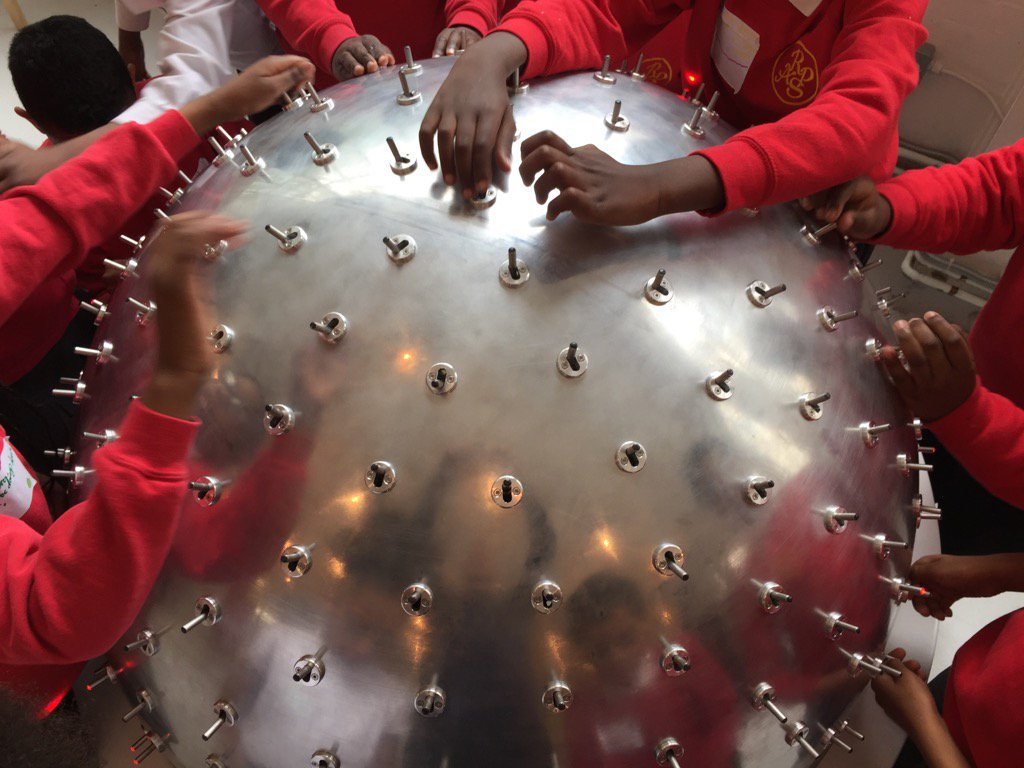
\includegraphics[width=8cm]{ioisphere}
\centering
\setlength{\belowcaptionskip}{-12pt}
\caption{iOi Sphere in action at the Institute of Imagination}
\label{fig:sphere}
\end{figure}

iOiSphere, commissioned by the Institute of Imagination and completed in 2017, acts as a digital fascinator for school visits. It is a 1-meter diameter hemisphere; the surface, of which, is covered in 202 toggle switches. Each individual custom designed toggle switch has an embedded LED and audio response, acting as both input and output. As a standalone artefact, iOiSphere hosts several games that are playable in parallel to encourage co-creative and casual play. Beyond the default behavior, a USB port in the side of the sphere allows pupils on school visits to upload  code that they have developed themselves to modify its behavior.  

The next stage in this research involves creating a web-based integrated development environment (IDE) with a simple visual scripting interface, a simulator of iOiSphere, and a small curriculum that contains tutorials on how to program the sphere. Programs created in the classroom using the IDE can then be downloaded as Arduino sketches and uploaded to the iOiSphere as part of the activities included in a school visit. A user-centered approach is key to avoid typical pitfalls in this field \cite{Hansen}. The impact of the engagement with iOiSphere will be measured through a small questionnaire integrated into the process of uploading a program to the sphere and with consideration for the stages outlined by Resnick for creative thinking \cite{Resnick:2007:IRN:1254960.1254961}.

\bibliographystyle{ACM-Reference-Format}
\bibliography{sample-bibliography}

\end{document}
